%FILE FOR RISK ANALYSIS
There are many risks and reasons why a project might fail or go bad, A change in organizational priorities is the most common reason. A change in project objectives is also common as poor communication and unclear risk definition.
	\begin{itemize}
		\setlength\itemsep{-0.3em}
		\item Unclear or shifting goals.
		\item lack of planning.
		\item lack of follow up.
		\item timing issues 
		\item Lack of risk management.
		\item Unsuitable tools.
		\item Too many unsuitable tools
	\end{itemize}

\noindent
For these reasons and many more, we’ve created an overall table with ratings which rate the opportunity/effect and risk.

\subsubsection{Scale} %SMALL HEADER
Ratings that can be seen below are from 1 to 9. Where 1 is low risk and 9 is high risk.\\
	
	
	% Please add the following required packages to your document preamble:
% \usepackage{graphicx}
% \usepackage[table,xcdraw]{xcolor}
% If you use beamer only pass "xcolor=table" option, i.e. \documentclass[xcolor=table]{beamer}
\begin{table}[!h]
\centering
\resizebox{\textwidth}{!}{%
\begin{tabular}{|l|
>{\columncolor[HTML]{9AFF99}}l |l|l|l|
>{\columncolor[HTML]{9AFF99}}l |
>{\columncolor[HTML]{9AFF99}}l |l|}
\hline
\cellcolor[HTML]{CBCEFB}Risk                                                                       & \cellcolor[HTML]{CBCEFB}Opportunity & \cellcolor[HTML]{CBCEFB}Effects & \cellcolor[HTML]{CBCEFB}Risk & \cellcolor[HTML]{CBCEFB}\begin{tabular}[c]{@{}l@{}}Measure to prevent /\\ Remedy it\end{tabular}                                                                 & \cellcolor[HTML]{CBCEFB}Change after & \cellcolor[HTML]{CBCEFB}Consequences afterwards & \cellcolor[HTML]{CBCEFB}Ultimate risk \\ \hline
\begin{tabular}[c]{@{}l@{}}A group member\\ lacks in work / failed\\ deadlines.\end{tabular}       & \cellcolor[HTML]{FFFC9E}4           & \cellcolor[HTML]{9AFF99}2       & \cellcolor[HTML]{FFCCC9}8    & \begin{tabular}[c]{@{}l@{}}Code of conduct created and\\ singed by everyone\end{tabular}                                                                         & 3                                    & 3                                               & \cellcolor[HTML]{FFFC9E}4             \\ \hline
\begin{tabular}[c]{@{}l@{}}Clear file locations\\ and easy to map.\end{tabular}                    & 3                                   & \cellcolor[HTML]{9AFF99}3       & \cellcolor[HTML]{FFFC9E}6    & \begin{tabular}[c]{@{}l@{}}Weekly document tracking\\ and documentation is taken.\end{tabular}                                                                   & 2                                    & 3                                               & \cellcolor[HTML]{9AFF99}3             \\ \hline
\begin{tabular}[c]{@{}l@{}}Behind schedule for\\ lack of knowledge or\\ confusion.\end{tabular}    & 4                                   & \cellcolor[HTML]{9AFF99}3       & \cellcolor[HTML]{FFCCC9}7    & \begin{tabular}[c]{@{}l@{}}Ask for help in time from\\ fellow group members or\\ teachers.\end{tabular}                                                          & 1                                    & 2                                               & \cellcolor[HTML]{9AFF99}2             \\ \hline
Running low on budget.                                                                             & 1                                   & \cellcolor[HTML]{FFFC9E}6       & \cellcolor[HTML]{9AFF99}5    & Budget is documented.                                                                                                                                            & 1                                    & 3                                               & \cellcolor[HTML]{9AFF99}1             \\ \hline
\begin{tabular}[c]{@{}l@{}}There is insufficient\\ communication in the\\ group.\end{tabular}      & 2                                   & \cellcolor[HTML]{9AFF99}3       & \cellcolor[HTML]{FFFC9E}6    & \begin{tabular}[c]{@{}l@{}}Meetings will be scheduled 2-3\\ times a week, minutes and\\ notes are taken and uploaded\\ up to date.\end{tabular}                  & 1                                    & 3                                               & \cellcolor[HTML]{9AFF99}3             \\ \hline
\begin{tabular}[c]{@{}l@{}}Clear results are\\ missing.\end{tabular}                               & \cellcolor[HTML]{FFFC9E}4           & \cellcolor[HTML]{FFFC9E}6       & \cellcolor[HTML]{FFCCC9}9    & \begin{tabular}[c]{@{}l@{}}The strip planning clearly\\ states which part you need to\\ complete to be on schedule\\ with each part of the project.\end{tabular} & 2                                    & 3                                               & \cellcolor[HTML]{FFFC9E}6             \\ \hline
\begin{tabular}[c]{@{}l@{}}Shortage in\\ components\end{tabular}                                   & 2                                   & \cellcolor[HTML]{FFCCC9}9       & \cellcolor[HTML]{9AFF99}3    & \begin{tabular}[c]{@{}l@{}}A delay in ordering or\\ receiving parts\end{tabular}                                                                                 & \cellcolor[HTML]{FFFC9E}6            & \cellcolor[HTML]{FFFC9E}6                       & \cellcolor[HTML]{FFCCC9}9             \\ \hline
\begin{tabular}[c]{@{}l@{}}The planning of\\ Fontys teaching\\ material is incorrect.\end{tabular} & \cellcolor[HTML]{FFFC9E}4           & \cellcolor[HTML]{FFFC9E}5       & \cellcolor[HTML]{FFCCC9}9    & Read documents carefully                                                                                                                                         & \cellcolor[HTML]{FFFC9E}4            & \cellcolor[HTML]{FFCCC9}7                       & \cellcolor[HTML]{FFCCC9}7             \\ \hline
\end{tabular}%
}
\caption{Risk analysis}
\label{Risk analysis}
\end{table}
	
%	\begin{figure}[!ht]
%		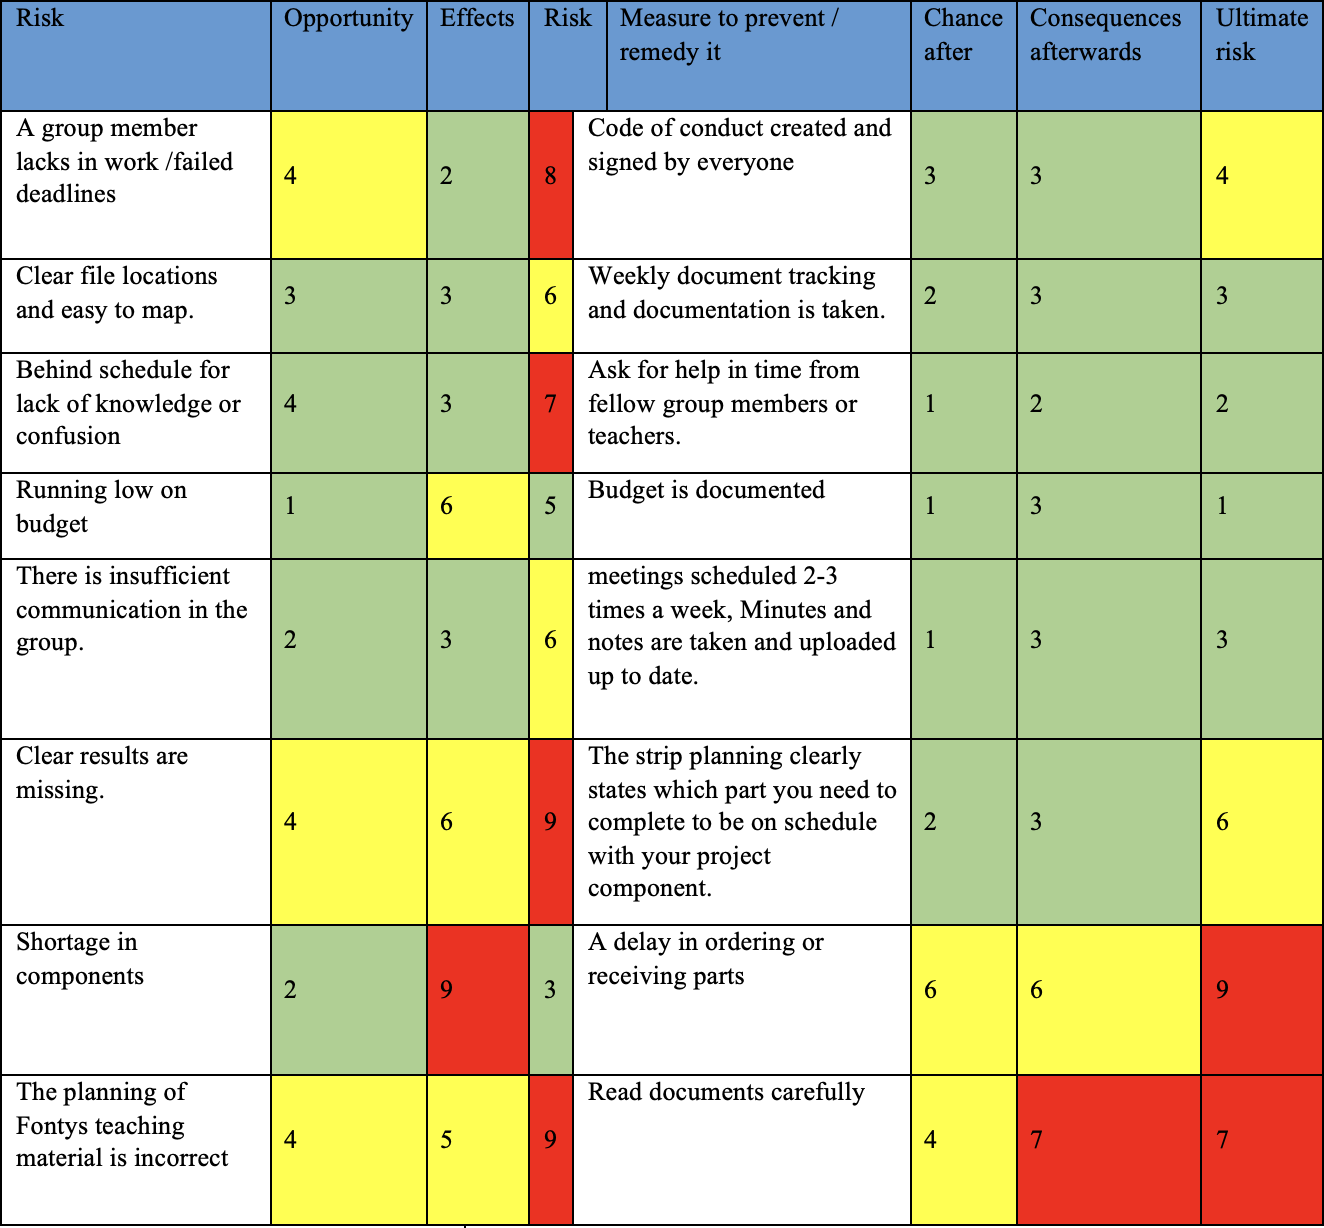
\includegraphics[scale = 0.4]{risk}
%		\caption{Table with risk rating}
%		\label{fig:risk}
%	\end{figure}